\documentclass[11pt]{article}

\usepackage[left=0.75in, right=0.75in, top=0.75in, bottom=0.75in]{geometry}
\usepackage{layout}
\usepackage{ucs}
\usepackage[utf8x]{inputenc}
\usepackage{titlesec}
\usepackage{graphicx}
\usepackage{amssymb}
\usepackage{amsmath}
\usepackage{dsfont}
\usepackage{float}
\usepackage{caption}
\usepackage{subcaption}
\usepackage{array}



\title{\textbf{TS225 TP}\\Compte rendu - Partie 3}
\author{Maxime PETERLIN - \texttt{maxime.peterlin@enseirb-matmeca.fr}\\
Gabriel VERMEULEN - \texttt{gabriel@vermeulen.email} \\\\{ENSEIRB-MATMECA, Bordeaux}}
\date{17 novembre 2014}


\begin{document}

\maketitle
\tableofcontents

\vspace{1.25cm}

\section{Introduction}

Le but de ce TP est l'implémentation d'algorithmes de traitement d'images permettant la détection et le rehaussement de contours. Les tests seront effectués sur l'image suivante.

		\begin{figure}[h]
			\centering
			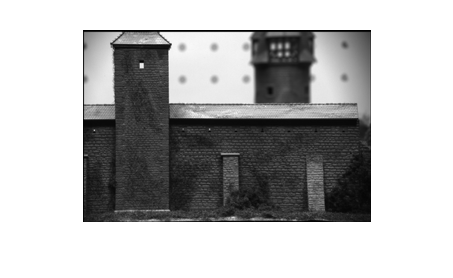
\includegraphics[scale=0.5]{img/batiment.png}
			\caption{batiment.bmp}
			\label{img1}
		\end{figure}
		

\newpage

\section{Détection de contours}
	
	\subsection{Calcul des composantes $\textbf{\textit{H}}_x^{1D}$ et $\textbf{\textit{H}}_y^{1D}$}
	
		On a 
		\[
		\begin{align}
			\textbf{\textit{S}}_x^{2D} &= \textbf{\textit{H}}_x^{1D} \otimes \textbf{\textit{H}}_y^{1D} = \frac{1}{2\sqrt{2}}[a_1\ b_1\ c_1]^T \otimes \frac{1}{2\sqrt{2}}[a_2\ b_2\ c_2].\\
			&= \frac{1}{8}\left( \begin{array}{ccc}
a_1a_2 & a_1b_2 & a_1c_2 \\
b_1a_2 & b_1b_2 & b_1c_2 \\
c_1a_2 & c_1b_2 & c_1c_2
\end{array} 
\right)= \frac{1}{8}\left( \begin{array}{ccc}
1 & 0 & -1 \\
2 & 0 & -2 \\
1 & 0 & -1
\end{array} 
\right)
		\end{align}
		\]
		\\
		
		Tout d'abord, comme $a_1a_2 = 1$, on a $a_1 \neq 0$ et $a_2 \neq 0$. Ainsi, $a_1b_2 = 0 \Rightarrow b_2 = 0$.\\
		Ensuite, on a $a_1a_2 + a_1c_2 = a_1(a_2+c_2) = 0$. $a_1 \neq 0 \Rightarrow a_2 + c_2 = 0$.\\
		$a_1a_2 - c_1a_2 = a_2(a_1-c_1) = 0$. Comme $a_2 \neq 0$, alors $a_1 - c_1 = 0$. En suivant le même raisonnement, on trouve $a_1-2b_1 = 0$.\\
		\\
		On pose alors $a_2 = 1$ et on en déduit ainsi que $\textbf{\textit{H}}_x^{1D} = \frac{1}{2\sqrt{2}}[1\ 0\ -1]$ et que $\textbf{\textit{H}}_y^{1D} = \frac{1}{2\sqrt{2}}[1\ 2\ 1]^T$.\\
		\\
		$\textbf{\textit{H}}_x^{1D}$ a pour but le calcul du gradient à une position donnée. A l'inverse du masque plus simpliste $[1 -1]$ qui calcule le gradient entre deux positions.\\
		$\textbf{\textit{H}}_y^{1D}$ permet de moyenner le calcul du gradient afin de ne pas être trop perturbé par le bruit tout en donnant un poids plus fort à la ligne du milieu.\\
	
	\subsection{Principe de fonctionnement du filtre de Sobel}
	
		Le filtre de Sobel est utilisé en traitement d'images pour la détection des coutours de ces dernières. Il va calculer, pour chaque pixel, la direction, ainsi que le taux de la plus forte variation d'intensité à l'aide de dérivées verticales et horizontales. Ces taux de variations soudains sont, a priori, les bords de l'image que l'on cherche à détecter.
	
	\newpage
	
	\subsection{Application des masques $\textbf{\textit{S}}_x^{2D}$ et $\textbf{\textit{S}}_y^{2D}$}
	
		\begin{figure}[h]
			\centering
			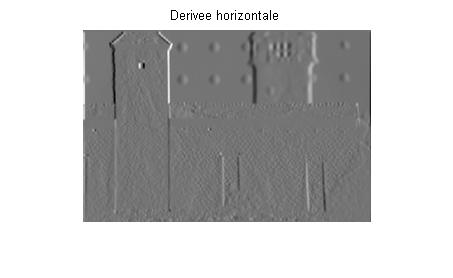
\includegraphics[scale=1]{img/derivee_horizontale.png}
			\caption{Application du masque $\textbf{\textit{S}}_x^{2D}$ sur batiment.bmp}
			\label{img1}
		\end{figure}
	
		\begin{figure}[h]
			\centering
			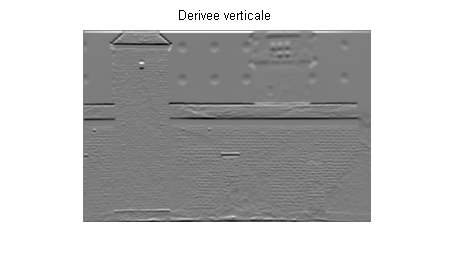
\includegraphics[scale=1]{img/derivee_verticale.png}
			\caption{Application du masque $\textbf{\textit{S}}_y^{2D}$ sur batiment.bmp}
			\label{img1}
		\end{figure}
	
	\subsection{Détection des contours}

		La détection des contours se fait par calcul, en tout point de l'image traitée, de la norme euclidienne du vecteur formé par les estimées des dérivées horizontale et verticale.\\
		Ainsi, soient $D_x = (a_{i,j})$ et $D_y = (b_{i,j})$ les matrices représentant l'image après l'application respective des masques $\textbf{\textit{S}}_x^{2D}$ et $\textbf{\textit{S}}_y^{2D}$.\\
		La matrice des normes euclidiennes considérées est donnée par $D_n = (\sqrt{a_{i,j}^2 + b_{i,j}^2})$
	
		\begin{figure}[h]
			\centering
			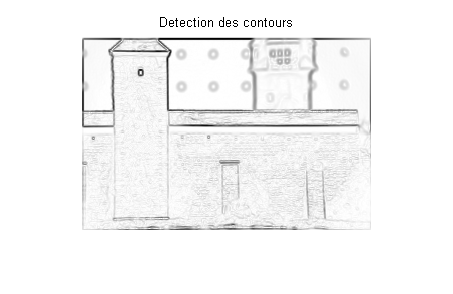
\includegraphics[scale=1]{img/detection_contours.png}
			\caption{Détection des contours de l'image batiment.bmp}
			\label{img1}
		\end{figure}
		
		\newpage

\section{Rehaussement}

	\subsection{Paramètre a}
	
		On cherche ici à determiner le paramètre a utilisé dans le masque 1D permettant de générer l'opérateur Laplacien L.\\
		On connaît les relations suivantes :\\
		\[ L = \left( \begin{array}{ccc}
1 & 1 & 1 \\
1 & -8 & 1 \\
1 & 1 & 1
\end{array} 
\right)
= \frac{\textbf{\textit{S}}_x^{2D} + \textbf{\textit{S}}_y^{2D}}{2}
\]
\[ \textbf{\textit{S}}_x^{2D} = (\textbf{\textit{S}}_y^{2D})^T = [1\ -2\ 1] \otimes [1\ a\ 1]^T
= \left( \begin{array}{ccc}
1 & -2 & 1 \\
a & -2a & a \\
1 & -2 & 1
\end{array} 
\right)
\] 
Ainsi,\\
\[ \frac{\textbf{\textit{S}}_x^{2D} + \textbf{\textit{S}}_y^{2D}}{2} = 
\left( \begin{array}{ccc}
1 & \frac{a-2}{2} & 1 \\
\frac{a-2}{2} & \frac{-2a-2a}{2} & \frac{a-2}{2} \\
1 & \frac{a-2}{2} & 1
\end{array} 
\right)
\] 
On en déduit donc que $a = 4$.\\
\\
Le premier masque 1D $[1\ -2\ 1]$ permet de détecter les contours tout en ayant un contraste plus fort (qu'un masque $[1\ 0\ 1]$ par exemple) au niveau du pixel considéré.\\
Le second masque 1D $[1\ 4\ 1]$ permet, comme pour l'opérateur de Sobel, de lisser la zone où l'on applique l'opérateur afin d'éliminer le bruit et de ne pas détecter les contours associés à ce dernier.\\

	\subsection{Application du masque L à batiment.bmp}
	
		Soit I l'image $batiment.bmp$, L l'estimation de l'opérateur Laplacien et $\alpha$ un paramètre de réglage arbitrairement fixé à 1. 
		Le masque est appliqué suivant la formule $I - \alpha \times I \otimes L$.

		\begin{figure}[h]
			\centering
			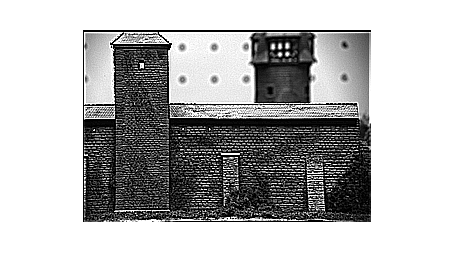
\includegraphics[scale=1]{img/rehaussement_contours.png}
			\caption{Rehaussement des contours de l'image batiment.bmp}
			\label{img1}
		\end{figure}
		
		Cette opération permet de soustraire l'image actuelle avec l'image représentant les contours. Ces derniers seront alors assombris par rapport à l'image originale. Le paramètre $\alpha$ permet de spécifier dans quelle mesure les contours doivent être rehaussés.
		

	\subsection{Propriété du Laplacien}
	
		Si on décompose L de la manière suivante :
		\[ L = \left( \begin{array}{ccc}
0 & 1 & 0 \\
1 & -4 & 1 \\
0 & 1 & 0
\end{array} 
\right)
+ \left( \begin{array}{ccc}
1 & 0 & 1 \\
0 & -4 & 0 \\
1 & 0 & 1
\end{array} 
\right),
\]
		on met en évidence la linéarité du Laplacien, ainsi que son invariance par rotation.

\end{document}
